\chapter{LoRa}

LoRa stands for \textbf{Lo}ng \textbf{Ra}nge. It is a transmission standard that aims at achieving long range reach with low power
consumption, most commonly used by the Internet of Things devices.
LoRa technology was first developed by Cycleo from Grenoble, France around 2010 with first prototypes implementing point-to-point communication for walkie-talkie and metering applications \cite{trinity_panel}. Later in 2012 the Cycleo team was aquired by Semtech, and released the chips for LoRa end devices and gateways \cite{origins}. [HERE TALK ABOUT LORAMAC AND PHYSICAL LAYER]\\

The open non profit organisation LoRa Alliance emerged in 2015\cite{alliance} [MB NOT REFERENCE JUST A WEBSITE]. 
It is an association of companies with Semtech being one of
its founding members \cite{alliance_founder} backing up the LoRaWAN protocol, insuring its
global presence and acceptance. The total number of members of the alliance has surpassed 500 in 2017 \cite{500_members}. Among the notable members are Cisco, Amazon and Alibaba \cite{alliance_members}.\\

One of the biggest contributors to the Lora Alliance project is The Things Network (TTN). TTN \footnote{https://www.thethingsnetwork.org/} is an open community of volunteers that took on an initiative to contruct and maintain LoRaWAN stations around the world to reach its global coverage. On their website they also provide tutorials and guides to help people deploy LoRaWAN gateways and nodes. 

\section{Basics}

Before diving into the specifics of LoRa and how it operates, let's have a look at the fundamental technologies and techniques behind it. \\

The most well known ways of transmitting information 
via electro-magnetical waves are AM and FM — amplitude and frequency modulation. In addition to radio broadcasting both these techniques have a range of applications such as radar, EEG, computer modems. When 
on is concerned with digital communications we want to 
encode ones and zeroes into the waveforms of the EM waves. For AM it is possible. \\

One of the main specifications about the proprietary standard LoRa is the one published by Semtech itself \cite{semtech_spec}. In the next few sections I will try to expand on the selected parts of it and explain them in detail.

\section{LoRa Physical layer}

\subsection{Shannon–Hartley theorem}

As the spec recognizes, an important starting point is the Snannon-Hartley theorem or also referred to as The Shannon limit - a significant milestone in information theory \cite{mit_article_on_shannon} . What it basically describes is the maximum data rate that a channel can have transmitted error-free in a particular bandwidth subject to noise. Here is the formula referenced by Semtech \cite{semtech_spec}, first introduced in the original paper \cite{shannon} by Claude Shannon:
\begin{equation}
    C = B \times log_2 (\frac{S}{N} + 1)
\end{equation}
where:
\begin{equation}
    C &- \text{channel capacity (in bits/s)}, \\
    B &- \text{channel bandwidth (in Hz)},\\
    S &- \text{average received signal power (in Watts)},\\
    N &- \text{average noise or interference power (in Watts)},\\ 
\end{equation}
Following the approximation from LoRa specification \cite{semtech_spec} assuming such noise that $\frac{S}{N} <<$ 1 applying the approximation to the algorithm:
\begin{equation}
    log_2(1 + \frac{S}{N}) &= \frac{ln(1+ \frac{S}{N})}{ln2} \approx \frac{1}{ln2}\times \frac{S}{N} \approx 1.443 \times \frac{S}{N} \approx \frac{S}{N} \\
\end{equation}
Subsequently we get:
\begin{equation}
    \frac{C}{B}& \approx \frac{S}{N} \\
\end{equation}
Which is equivalent to:
\begin{equation}
    \frac{N}{S} & \approx \frac{B}{C}
\end{equation}



As can be seen from the formula, to transmit error free data with noise-to-signal ratio fixed, one only needs to increase the signal bandwidth \cite{semtech_spec}.

\subsection{Direct Sequence Spread Spectrum (DSSS)}

Direct Sequence Spread Spectrum is a signal transmission technique based on increasing the bandwidth of the original data generated by the sender by multiplying it by the spreading code — a sequence of bits, also known as chips \cite{dsss_article}. [POSSIBLY INCLUDE DIAGRAMS TO DEMOSTRATE ECNODING AND DECODING] The signal is decoded at the receiver by again multiplying the signal with
the same spreading sequence of bits \cite{dsss_article}. One of the disadvantages of this transmission technique is that it is too power hungry and demanding for low-power devices or networks with small resources \cite{semtech_spec}.

\subsection{LoRa Spread Spectrum (Chirp Spread Spectrum)}

CSS is a modulation technique that has been around since 1940s \cite{semtech_spec} with 
applications in naval and air military and also observed in fauna \cite{origins}. What makes CSS different from other Spread Spectrum techniques (despite some claiming it to be a subtype of DSSS \cite{orthogonality_description}) is the fact that it is resistant to multi-path fading and Doppler effect while having relatively moderate transmission power demands \cite{semtech_spec}. \\

According to IEEE standard for information technology \cite{ieee_2007} "A chirp is a linear frequency modulated pulse. It could be thought of as sweeping the band at a very high speed. The type of CSS system defined for this standard uses patterns of smaller chirps, or ’sub chirps’, to build one larger chirp symbol." \\

When describing CSS symbols we are mainly concerned with 4 parameters. 
Spreading factor ($SF$), minimal frequency $f_{min}$, maximal frequency $f_{max}$ and the input bits. Generation of a CSS symbol starts at the starting frequency $f_0$ lying between $f_{min}$ and $f_{max}$ as can be seen on the figure \ref{fig:slope}. The difference between $f_{min}$ and $f_{max}$ (i.e. $f_{max} - f_{min}$) is called bandwidth — B. $f_0$ represents the input information of $SF$ bits. Thus the symbol duration can be calculated using this formula from Application Note Semtech AN1200.22 \cite{semtech_spec}: 
\begin{equation}
    T_S = \frac{2^{SF}}{B} 
\end{equation}

% Spreading factor determines the number of bits to be encoded in a signal \cite{sf}

% LoRa employs six spreading factors from 7 to 12 to provide orthogonality in data transmission (collision-free) occurring on the same frequency.  SF determines the chirp rate — change in frequency with respect to time which is the slope on \ref{fig:slope}{}

\begin{figure}[h!]
  \centering
  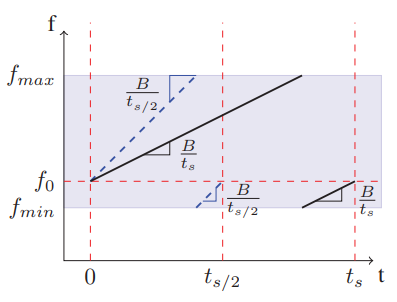
\includegraphics[scale=0.5]{figures/slope.PNG}
  \caption{Graphical representation of the frequency in time for
two CSS symbols with 2 different spreading factors. Source: \cite{slope_diagram}}
  \label{fig:slope}
\end{figure}

% An advantage of LoRa spread spectrum is that timing and frequency offsets between transmitter and receiver are equivalent, greatly reducing the complexity of the receiver design. \cite{semtech_spec}  

\subsection{Spreading factors}

According to the spec \cite{semtech_spec}
LoRa employs 6 spreading factors from 7 to 12. Spreading factor value is the number of bits a symbol can represent \cite{sf_article} and looking at figure \ref{fig:slope} it determines the rate of the frequency change in a sweep. 

Spreading factors allow different signals to be transmitted
over the same channel at the same time. As the specification claims it is possible due to the orthogonality of CSS signals of different spreading factors to each other \cite{semtech_spec}.
Despite the claim of the orthogonality feature of spreading factors in CSS signals, it has been shown to be quasi-orthogonal and the decoding of signal at the receiver
can be disrupted under certain conditions for example if the power of the interfering signal is stronger than the one to decode \cite{imperfect_1}.

\section{LoRaWAN}

On top of the physical layer there needs to be a protocol.
And such is the LoRaWAN layer backed by the LoRa Alliance. 
As the LoRa Alliance itself states on its website 
\cite{lora_alliance_about_lorawan} LoRaWAN is 
"a networking protocol designed to wirelessly connect battery operated 
‘things’ to the internet in regional, national or global networks".

\subsection{Network Topology}

The LoRaWAN standard is based on a star topology.
Multiple end devices (nodes) communicate with a gateway (base station) and multiple gateways communicate with the main network server as demonstrated in the figure \ref{fig:star}. Here gateway acts as an agent between the nodes and the internet, translating Radio Frequency messages into Internet Protocol packets and vice-versa \cite{lora_alliance_about_lorawan}.
One gateway can typically cover a range of hunderds of meters to tens of kilometers with up to millions of end devices \cite{doppler}.

\begin{figure}[h!]
  \centering
  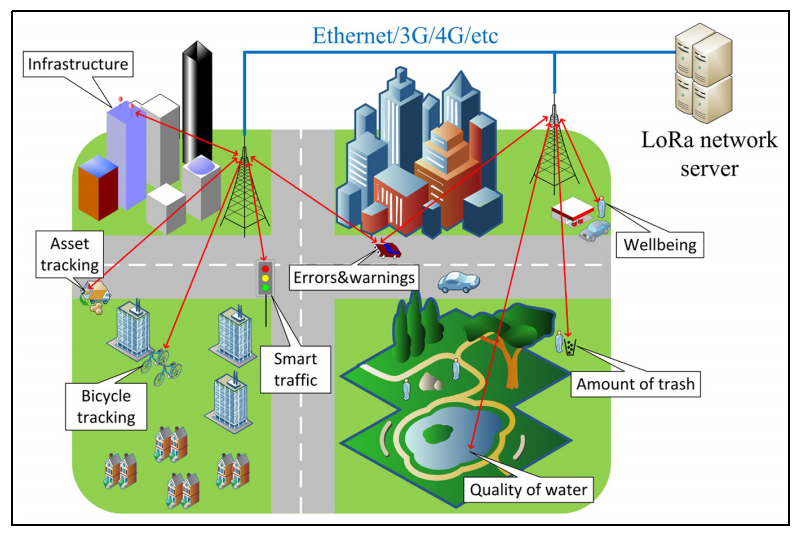
\includegraphics[scale=0.4]{figures/start-topology.PNG}
  \caption{LoRaWAN nodes and gateways connected to a LoRa server Source: \cite{doppler}}
  \label{fig:star}
\end{figure}

\newpage

\subsection{Multiple Access Control (MAC) scheme}

LoRaWAN implements ALOHA protocol where any device can wake up and transmit a message regardless of time. We are concerned with the messages between a LoRaWAN device and a gateway (base station). Requests from a node to a gateway are called uplink messages, and the responses are called downlink messages.  
The communication scheme has an uplink-centric design and 
LoRaWAN mandates this design for all devices implementing the protocol \cite{simulator}. In the figure \ref{fig:class A} one can see the typical cycle a node goes through while communicating with a particular gateway. The receive windows are allocated periods of time when the node is expecting 
a downlink response that should follow its uplink request.

\begin{figure}[h!]
  \centering
  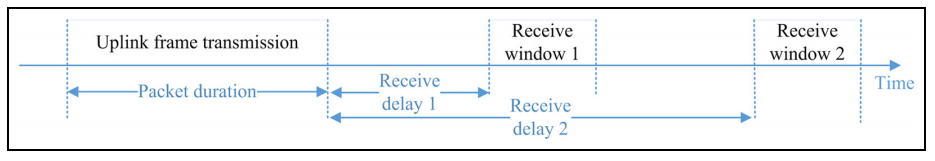
\includegraphics[scale=0.5]{figures/class A.PNG}
  \caption{Class A type LoRaWAN device scheduling of receive slots for downlink messages. Source: \cite{doppler}}
  \label{fig:class A}
\end{figure}

There are 3 different device types based on the way to schedule the receive window slots for downlink communication: class A, B and C. Support for class A (demonstrated in the figure \ref{fig:class A} above) is compulsory with B and C being extensions to it. Class A devices schedule 2 receive windows following an uplink transmission, class B devices open receive windows periodically and class C devices listen for downlink messages continuously unless they are transmitting \cite{lora_alliance_spec}. 

\subsection{Duty cycle}
For each band LoRaWAN devices operate in, they need to comply with the industrial, scientific and medical (ISM) regulations often set by the local government \cite{duty_cycle}. These include the duty cycle limitation that determines amount of time a device can be active within a bandwidth. For example in Europe the duty cycle standards are set by the 
European Telecommunications Standards Institute (ETSI) —  "the recognized regional standards body dealing with telecommunications, broadcasting and other electronic communications networks and services.", as their website  \cite{about_etsi} states.\\ 

What duty cycle basically controls is the fraction of time a device can be active on a particular sub-band (potentially on multiple channels) \cite{duty_cycle}. For example if the channel in 
question is used for 1 time unit for every 10 time units,
the device using it has a duty cycle of 10\%. If we take into account multiple channels (within one sub-band), then we count in the total fraction of time these channels are being used by the device \cite{duty_cycle}. [INFO ABOUT section 7.2.3 of the ETSI EN300.220 standard]

\section{NOMA}
 
 Non-Orhogonal Multiple Access (NOMA) scheme is a relatively new concept first introduced in this publication \cite{noma_original} in 2013. As opposed to orthogonal
frequency division multiplexing (OFDM), NOMA decodes multiple incoming signals, occupying the same time 
or frequency resources, utilizing the power or code domain \cite{noma_imperial}. [DIAGRAM FROM TUTORIAL]. In the power domain implementation of NOMA the decoding is achieved via successive interference cancellation (SIC) based on the 
different power levels of the incoming signals \cite{noma_imperial} \cite{noma_original} ??? .\\ 

Despite the original paper \cite{noma_original} focusing on the downlink NOMA
implementation (i.e. end-device/node being the receiver in question), we are interested in the uplink communications and thus the workings of NOMA at the gateway. 
  
%  As the name NOMA suggests, it it does not utilizes the orthogonality of 
%  , but instead decodes multiple incoming signals based on the 
 
 
\chapter{Simulation Framework}

In order to simulate a LoRaWAN network I have decided to pick one described in this paper \cite{simulator}. The developers of the paper have closely followed guidelines from The Things Network. The simluation code is published in github \cite{simulator_github}. The developers have decided to simulate the LoRaWAN network via the \texttt{SimPy} python library which "is a process-based discrete-event simulation framework based on standard Python"\cite{simpy}. The simulation is mainly driven through continuous yielding of appropriate generator functions. A potential improvement to the code would be introduction of some sort of parallelisation.


\subsection{Architecture}

The simulation is based on the LoRaWAN architecture of star-toppology network with mutiple nodes connected to a single gateway as already described above and in the figure \ref{fig:star}. The simulation supports only one gateway, so among other improvements would be introduction of multiple gateways in the simulated area. \\

In the following figure \ref{fig:architecture} is the scheme describing relations between the most relevant simulation python classes (along with their names).

\begin{figure}[h!]
  \centering
  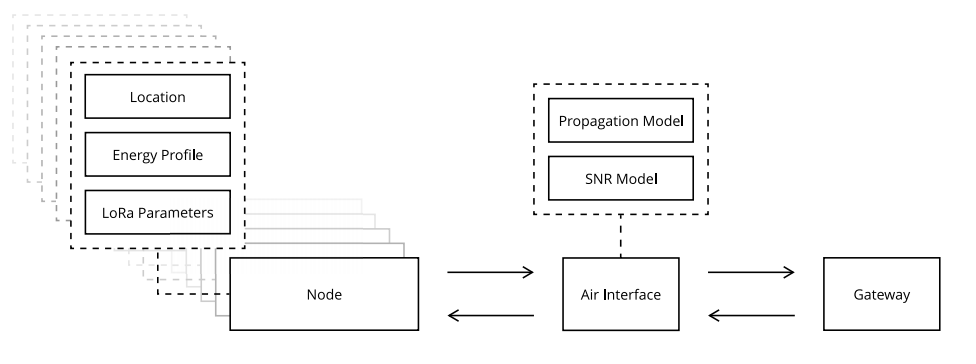
\includegraphics[scale=0.5]{figures/architecture.PNG}
  \caption{Interaction between python classes: \cite{simulator}}
  \label{fig:architecture}
\end{figure}

\subsection{Nodes}

As can be seen from the figure \ref{fig:architecture} the \texttt{Node} object is characterized by the \texttt{Location}, \texttt{Energy Profile} and \texttt{LoRa Parameters} objects (among others) passed to its constructor during initialization as parameters.\\

\texttt{Location} as its name suggests, simply holds the coordinates for a particular Node. The simulation assumes a rectangular cell, and the particular node location is typically randomly selected within the bounds of that rectangle. \\

\texttt{Energy Profile} holds information about the different power states and their duration in the execution loop of communication between a node and its respective gateway (sketched above in \ref{fig:class A}). The energy profile used in the original paper \cite{simulator}, as the authors stated was motivated by the energy consumption analysis of another project — LoRaWAN implementation for the EFM32 Happy Gecko develop board \cite{energy_profile}. The energy profile used is displayed in the figure below:

\begin{figure}[h!]
  \centering
  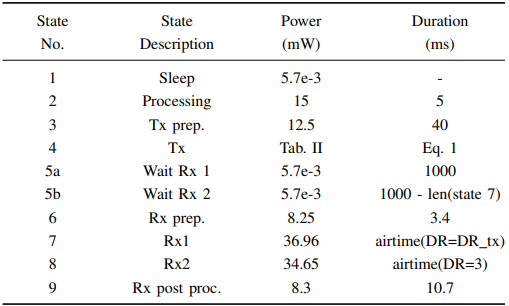
\includegraphics[scale=0.7]{figures/energy_profile.PNG}
  \caption{Energy Profile devised from \cite{energy_profile}. Source: \cite{simulator}}
  \label{fig:energy_profile}
\end{figure}\\

The effect of implementing this energy profile can be seen in the figure \ref{fig:power_states} below; it displays, how the power states of a node develop in time:

\begin{figure}[h!]
  \centering
  \hspace*{-1cm}  
  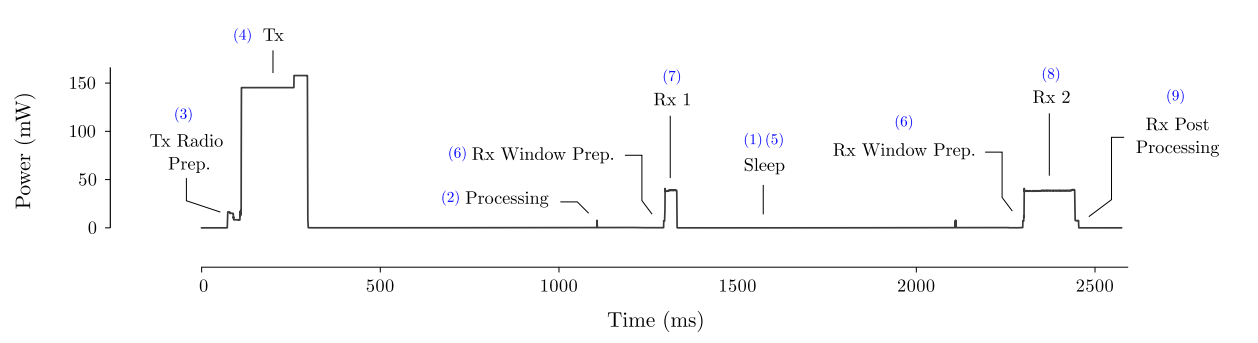
\includegraphics[scale=0.5]{figures/class A 2.PNG}
  \caption{Power states of a LoRa node simulated in \cite{simulator}}
  \label{fig:power_states}
\end{figure}\\

\texttt{LoRa Parameters} object holds information about the configuration of the uplink packets that the Node is going to send, such as its spreading factor, frequency (channel) and transmission power. These are the factors that play a crucial role in the resulting energy consumption at the node [CITE THAT???] .

\subsection{AirInterface}

\texttt{AirInterface} is the object via which \texttt{Node} and \texttt{Gateway} communicate. It processes the packets "in the air" and determines their airtime as well as simulating collisions between packets. 2 important objects that define it are \texttt{Propagation Model} and \texttt{SINR Model}.\\

\newpage

\texttt{Propagation Model} calculates the path loss 
of a signal traveling in the channel through the air.
the formula is defined in the original paper \cite{simulator} :
\begin{equation}
    PL(d) = PL(d_0) + 10n\times log\frac{d}{d_0} + X_{\sigma} [dB]
\end{equation}

Where the following parameters are used (parameters are taken for granted by the authors \cite{simulator} from another source \cite{propagation_model_parameters} [MORE DETAIL ON WHY AND HOW]):
\begin{align*}
     d_0 & = 1000 \text{m}\\
     PL(d_0) & = 128.95 \text{dB}\\
     X_{\sigma} & = 7.8 \text{dB}\\
     n & = 2.32\\
\end{align*}

The \texttt{SINR Model} is implemented similarly to how \texttt{SNR Model} was implemented in the original simulator. The model calculates signal-to-interference noise ratio (SINR) for the received signal strength values of packets in the air according to this formula [CITE WIKIPEDIA???]:
\begin{equation}
    \text{SINR}(x) = \frac{P}{I + N}
\end{equation}
where:
\begin{align*}
     P &- \text{power of the examined signal}\\
     I &- \text{total interference from weaker signals in the air}\\
     N &- \text{ noise floor}\\
\end{align*}

The interference is only calculated from the weaker signals, since we're assuming that NOMA is enabled at 
the gateway and thus all the stronger signals would be
decoded apriori \cite{noma_original}.\\

\texttt{SINR Model} also calculates throughput from SINR values. The need for throughput metric will be explained below. This formula [CITE WIKI???] is used:

\begin{align*}
    \text{throughput} = \text{$log_{2}$}(\text{sinr} + 1)
\end{align*}

Collision model is not implemented as a separate object but through a collection of functions in \texttt{Air Interface}. The model implementation is motivated by the authors \cite{simulator} by the findings from another paper \cite{collision_conditions}, that looks at how reception overlap, carrier frequency, spreading factor and power can create conditions for a packet collision. The authors \cite{simulator} also assume that signals with different spreading factors are practically orthogonal and can be demodulated without colliding.

\subsection{Gateway}

\texttt{Gateway} object is responsible for receiving 
the uplink packets from the \texttt{Air Interface}. In order for a packet to come through it must not collide and have  a signal strength above that of gateway's specified sensitivity. In the original simulator \cite{simulator} \texttt{Gateway} is also responsible for executing the ADR algorithm. ADR is the algorithm, devised to minmize the energy consumption at nodes, operating mainly by estimating the appropriate TP and SF values for each uplink packet and sending them to the respective node (that sent the packet) via a downlink frame \cite{simulator}. The node that uses these values until a next update from the gateway. In the original simulator these values are calculated based on the SNR values of the received frames. 
[INPUT DETAILS ON ADR and ADR itself maybe] \\

In this project, however we are not going to implement any form of ADR and instead apply reinforcement learning tecnhiques to 
decide on appropriate \texttt{LoRa Parameters} values for uplink frames.


% Due to the SF orthogonality assumption, the gateway can simultaneously receive up to 8 different packets on separate channels. [FALSE???]

\chapter{Reinforcement Learning} 

Reinforcement Learning has recently seen a rise in popularity after
the success of DeepMind in 2016 after AlphaGo beat the Korean 9-dan professional Go player \cite{alpha_go_lee_sedol} and after more recently OpenAI beat a team of professionals in a Dota 2 match \cite{dota}.\\

Reinforcement Learning (RL) typically focuses on the problems of agents within some environment. The agents can act upon the environment with some goal in mind (e.g. robot playing chess). The policy of that agent (i.e. how it decides to act under certain conditions (e.g. coordinates on a map, temperature, board game position)) is the component, not specified by the programmer but instead learnt by the agent via trial-and-error interactions with the environment over the learning period. Thus RL often reduces to a problem of learning the optimal policy in the context of a particular application. [CITE ME???] \\

This closed loop can be demonstrated as in the figure \ref{fig:closed_loop} below, where an agent subject to state $S_{t}$
and reward $R_{t}$ takes an action $A_{t}$ which leads to a new
state $S_{t+1}$ and a new reward $R_{t+1}$:

\begin{figure}[h!]
  \centering
%   \hspace*{-1cm}  
  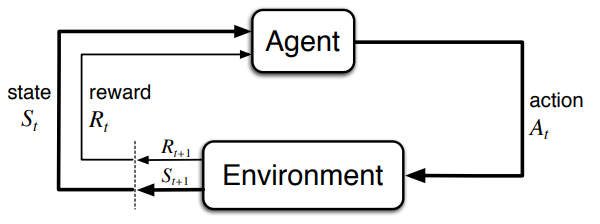
\includegraphics[scale=0.7]{figures/closed_loop.PNG}
  \caption{Closed-loop of reinforcement learning. Source: \cite{sutton_barto}}
  \label{fig:closed_loop}
\end{figure}\\  

\section{Terminology and symbols}
Here I'll explain the main bulk of terminology specific to reinforcement learning that we'll need for the rest of this chapter.\\

Rewards, Action, States, Policy, Value function [DO LATER]
 
\section{Markov Process}

Markov Chain is essentially a way to model stochastic processes with
particular properties. As the name suggests it is a chain of states
that describe the process we are modeling. Using an exmaple from this article \cite{markov_chain_article}, if we are to model weather at a particular region on a daily basis, we could have 2 states: Sunny and Rainy. Now what interests us are the transitions between these 2 states. We could model them as a simple random process such that the probability of it being Sunny after being Rainy was 0.5 and the probability of it being Rainy after being Sunny was 0.1. Furthermore if we assume the \textbf{memorylessness} property of this model i.e. that the weather tomorrow is \textbf{independent} of the weather yesterday and only depends on the weather today then we could effectively derive the other 2 missing probabilites for the weather staying Sunny (1 - 0.1 = 0.9) or Rainy (1 - 0.5 = 0.5) for 2 days in a row \cite{markov_chain_article}.

\begin{figure}[h!]
  \centering
%   \hspace*{-1cm}  
  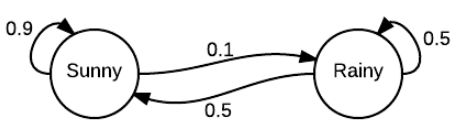
\includegraphics[scale=0.7]{figures/markov_weather.PNG}
  \caption{Closed-loop of reinforcement learning. Source: \cite{markov_chain_article}}
  \label{fig:weather}
\end{figure}

Thus we can describe a Markov process through a set of states S and a probability transition matrix P satisfying the \textbf{Markov property}
(memorylessness) [CITE]:
\begin{equation}
    P_{ss'} = P[S_{t+1} = s' | S_{t} = s]\\
    \sum_{s' \in S} P_{ss'} = 1
\end{equation}

\section{Markov Reward Process}
Markov Reward Process is a Markov Process that 
has a reward value tied to each state transition[CITE]. We can describe these rewards through another matrix R such that:
\begin{equation}
    R_{s} = E[r_{t+1} | S_{t} = s]
\end{equation}
This is the reward that the agent leaving state s receives upon transitioning at timestep $t+1$.\\

The process is also defined by a discount factor $\gamma \in [0, 1]$. We need it to define the return value which is the estimated sum of all rewards starting from time-step t as such:
\begin{equation}
    R_t = r_{t+1} + \gamma r_{t+2} + \gamma ^2 r_{t+3} + ... = \sum^{\infty}_{k=0}\gamma^{k}r_{t+k+1} 
\end{equation}

The discount factor allows the agent to put different weight on immediate and distant rewards,
with small $\gamma$ being more concerned with immediate results and large $\gamma$ looking far into the future. 

% [WHY DISCOUNTING IS A GOOD IDEA SLIDE 56 https://materials.doc.ic.ac.uk/view/2021/70028/Course\%20Material/7]
\subsection{State Value Function}
As the definition from lectures states: "The state value function v (s) of an MRP is the expected return R
starting from state s at time t":

\begin{equation}
    v(s) = \EX[R_t | S_t = s]
\end{equation}

If we expand the $R_t$ term and applying the Tower Rule and Law of Total we will eventually [INPUT derivation] get 

\begin{equation}
    v(s) = \EX[r_{t+1} + \gamma v(S_{t+1})| S_t = s] = R_s + \gamma \sum_{s' \in S} P_{ss'}v(s')\\
\end{equation}

And applying this to n states
\begin{equation}
    \textbf{v} = R + \gamma P \textbf{}
\end{equation}

where the vector \textbf{v} is n-dimensional.\\

A direct solution to this would be 
\begin{equation}
    \textbf{v} = (\bbone - \gamma P)^{-1}R
\end{equation}

But since matrix inversion is computationally very expensive it is often not feasible to find \tetxbf{v} that way for small MRPs. We will look into iterative solutions
for this problem: Dynamic programming, Monte-Carlo evaluation and Temporal Difference Learning.

\subsection{Policy}
According to the definition from the lecture: "A policy $\pi(a, s) = P[A_t = a | S_t = s]$ is the conditional probability distribution to execute an action $a \in A$ given that one is in state $s \in S$ at time t"

\section{Markov Decision Process}
We can now define what Markov Decision Process is, it is defined by a State Space S; action space A, transition probablity matrix $P^{a}_{ss'} = p(s_{t+1}| s_t, a_t)$, discount factor $\gamma \in [0, 1]$, reward function $R^{a}_{ss'}$ and policy $\pi$

\subsection{Value Function}
According to the definition from lectures: Value function for MDPs is:

\begin{equation}
    V^{\pi}(s) = \EX_{\pi}[R_{t} | S_t = s] = \EX[\sum^{\infty}_{k=0} \gamma^k r_{t+k+1} | S_t = s]
\end{equation}

"where $R_t$ is a discounted total return and the $r_{t+k+1}$" are immediate rewards.

\begin{equation}
    V^{\pi}(s) &= \EX_{\pi}[R_{t} | S_t = s] \\ 
    &= \EX[\sum^{\infty}_{k=0} \gamma^k r_{t+k+1} | S_t = s] \\
    &= ... \\
    &= \sum_{a \in A} \pi(s, a) \sum_{s' \in S} P^{a}_{ss'} (R^{a}_{ss'} + \gamma V^{\pi}(s'))
\end{equation}

"Thus we can see the self-consistency of the MDP value function and crucially $V^{\pi}$ has a unique solution"

\subsection{Policy Evaluation}
"Policy Evaluation is the computation of a Value function values for an arbitraty policy". One such evaluation method is Iterative Policy Evaluation where Bellman's equation is sytematically applied over and over again until hopefully Value Function converges for each state 

\subsection{State Action Value Function}
According to lecture "State Action Value Function defines How good is it to be in a given state and take a given action when you follow a policy $\pi$:

\begin{equation}
    Q^{\pi}(s, a) = \EX[R_t | S_t = s, A_t = a] = \EX[\sum^{\infty}_{k=0} \gamma^k r_{t+k+1} | S_t = s, A_t = a]
\end{equation}

And we can also derive the relationship between the state value and state-action value functions:

\begin{equation}
    V^{\pi}(s) = \sum_{a \in A} \pi(s, a) Q^{\pi}(s, a) 
\end{equation}

\subsection{Optimal Value and Optimality equations}
If we are to optimize the state value function V we are to determine the optimal ploicy. According to lectures Optimal Value Function is:
\begin{equation}
    V^*(s) = \max_{\pi} V^{\pi}(s)   \forall s \in S
\end{equation}
And respectively for the state-action value function (input) 

Applying to previous equation (4.9):
\begin{equation}
    V^*(s) = \max_{a}\sum_{s'} P^{a}_{ss'} (R^{a}_{ss'} + \gamma V^{*}(s'))
\end{equation}

Respectively for the state-action value function:
\begin{equation}
    Q^*(s, a) = \sum_{s'} P^{a}_{ss'} (R^{a}_{ss'} + \gamma Q^{*}(s', a'))
\end{equation}

\subsection{Assumptions}

Applying the Bellman Optimality Equation is one way to solve the problem of finding the optimal policy. But this relies on 3 assumptions: the environment model is well-known, we have computational resources to brute force the solution and of course the Markov property. So as often happens approximate solutions are searched.

\subsection{Convergence Proof}
"Theorem (Bellman Optimality Equation convergence theorem):\\

For an MDP with a finite state and action space:\\
 - The Bellman Optimality Equations have a unique solution and the values produces by the value iteration converge to the solution of  the Bellman equations"\\
 
 This can be proved through a Contraction Mapping Theorem.

\section{Dynamic Programming}
Dynamic Programming typically refers to a set of algorithms targeted at solving problems within well-defined systems such as Markov Decision Process. [CITE] 

The term dynamic programming (DP) refers to a collection of algorithms that can be used to compute optimal policies given a perfect model of the environment as a Markov Decision Process (MDP). [CITE]

\subsection{Policy Improvement Theorem}

As the lecture states the theory is as follows:\\\\

"Let $\pi$ and $\pi'$ be any two deterministic policies such that $\forall s \in S$"

\begin{equation}
    Q^{\pi}(s, \pi'(s)) \geq V^{\pi}(s).
\end{equation}

"Then $\pi'$ must be as good or better than $\pi$":
\begin{equation}
    V^{\pi'}(s) \geq V^{\pi}(s), \forall s \in S
\end{equation}

The theorem can be proved in a series of expansions [EXPAND ON THAT, CITE]

\subsection{Policy Iteration}

As the lecture notes state:

"Once a policy, $\pi$ , has been improved using $V^{\pi}$ to yield a better policy $\pi'$, we can compute $V^{\pi'}$ and improve it again to $\pi''$, to yield an even better $V^{\pi''}$. We can thus obtain a sequence of monotonically improving policies and value functions. This way of finding an optimal policy is called policy iteration."

\subsection{Bellman's Principle of Optimality}

As the lectures states Bellman's Principle of Optimality:\\

A policy $\pi(a, s)$ achieves the optimal value from state $s$, \vpidash{s} = $V^{*}(s)$, if and only if:\\ 
1) For any state $s'$ reachable from s, i.e. $\exists a : p(s', s, a) > 0$\\
2) $\pi$ achieves the optimal value from state s', \vpi{s'} = \voptimal{s'}
 
 \newpage
 
\subsection{Policy Iteration Algorithms}

\begin{figure}[h!]
  \centering
%   \hspace*{-1cm}  
  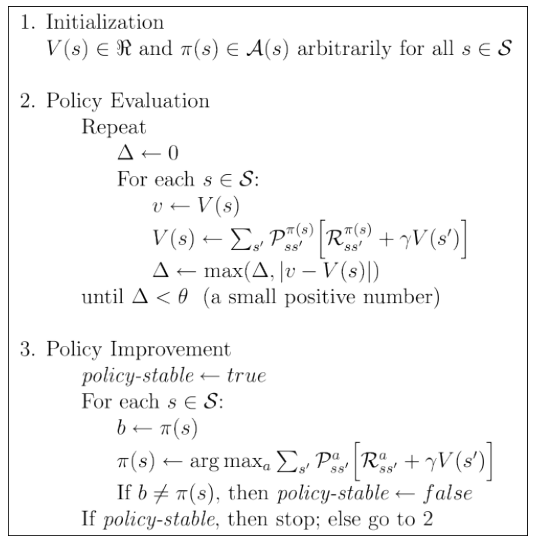
\includegraphics[scale=0.5]{figures/policy_iteration_algorithm.PNG}
  \caption{Policy Iteration Algorithm; Source: Lecture}
  \label{fig:pia}
\end{figure}

\subsection{Value iteration}

There are multiple ways to stop the iteration: $\epsilon$-convergence of value function or stopping after k iteratoins, or even just after one sweep of state space $S$ turning Bellman Optimality Equation into an update rule. 

\begin{figure}[h!]
  \centering
%   \hspace*{-1cm}  
  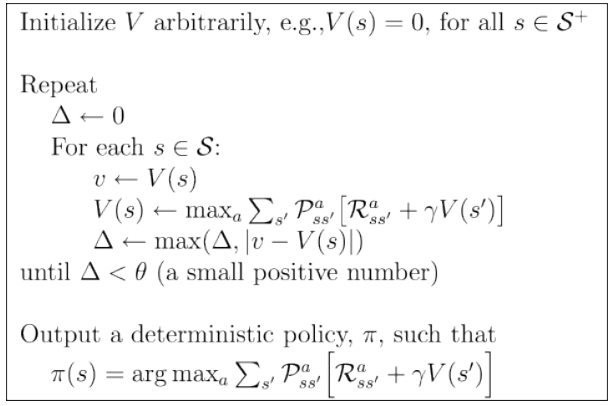
\includegraphics[scale=0.5]{figures/value_iteration_algorithm.PNG}
  \caption{Value Iteration Algorithm; Source: Lecture}
  \label{fig:via}
\end{figure}

\subsection{What DP gives us and what are its limits}

DP works well for moderate not resource hungry type of problems and suffers from the curse of dimensionality once the complexity increases. It also requires full knowledge of the Markov Decision Process which is not always available in pratice. Despite that it introduces a useful concept: "Bootstrapping" i.e. "updating values estimates based on other estimates" [LECTURE/BARTO] So these are the issues that Model Free Control learning addresses.


#######################################################

\section{Model-Free Learning}
Now we are going to learn to estimate and optimize our value function with an unknown MDP unlike in Dynamic Programming. 

\subsection{Monte Carlo methods}

MC methods learning directly from episodes of experience,
without MDP knowledge, episodes are complete, so no bootstrapping is necessary. The basic idea nehind it is calculating mean return of the episodes, but under the assumption that traces of episodes end in a terminal state.[CITE]

\subsection{MC Policy evaluation}

\begin{figure}[h!]
  \centering
%   \hspace*{-1cm}  
  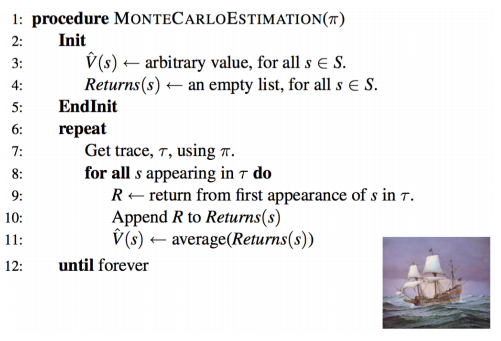
\includegraphics[scale=0.5]{figures/mc_policy_evaluation.PNG}
  \caption{MC Policy Evaluation Algorithm; Source: Lecture}
  \label{fig:via}
\end{figure}

Here you can see that value function is approximated with an average returns of states. This is a First-Visit MC algorithm, so only the first occurence of a state is counted toward the estimate. In Every-visit MC algorithm every occurence is recorded.[CITE]



\subsection{Batch & Online}


\section{Monte-Carlo}
\section{Temporal Difference}
\section{On and Off policy}
\section{Q-Learning}
\chapter{Learning Model}
\section{Distributed Learning}

The ideal situation would of course be having one learning agent 
per LoRa node so they could learn a policy specifically suited for
that one node. But the case is that typically nodes located 
near each other can benefit from one policy [CITATION or EXPERIMENT]
so in order not to waste memory on slightly different models 
for nodes located near each other nodes can be grouped into clusters
and share learning weights.



Despite first prototypes starting with 

\section{LoRa State}
\section{LoRa Action}
\section{LoRa Reward}

